%!TEX root =  ../main.tex

\subsection{Zeros}

\objective{Graph, read, and produce rational functions}


A rational function is one defined by $\frac{f(x)}{g(x)}$ where $f(x)$ and $g(x)$ are both
polynomials.  Rational functions exhibit some common behaviors with polynomials, 
such as $x$-intercepts and one $y$-intercept.  But they also tend to have vertical and
horizontal asymptotes.  The most basic rational function --- $\frac{1}{x}$ --- is, in fact,
a hyperbola, with two branches.  But rational functions can have many more than two
branches, or even just have one.


There are three things one could consider with regard to 0 and a given rational function.
First, the entire quotient could be 0, which would make $x$-intercepts.  Fortunately,
a quotient is only equation to zero when the numerator is equal to zero, meaning
we only need to find when top equation's zeros to find the whole equation's.

When the denominator is equal to zero, much more bizarre behavior emerges.  A vertical
asymptote will occur, though it is not immediately clear if the left and right limits will be
to opposite infinities, or to the same one.  Factoring will make it clear: if the term
has an even multiplicity, the asymptote will be followed to the same infinity.  Otherwise,
one sided-limit will be $\infty$ and the other $-\infty$.

Lastly, we should consider what happens when we make the argument 0.  A $y$-intercept
is always a coordinate with the appearance $(0,y_0)$, so plugging in 0 is an efficient way
to find it.

Each of these three techniques for various ``zero's'', assumes that it is not occurring when
function is in an indeterminate form.  Holes and asymptotes can prevent intercepts from 
actually occurring, and obfuscate one another

\subsection{Horizontal Asymptotes}
If a rational function looks like a fraction, a ratio, a quotient, that's because it is!  Just as
a polynomial looks more and more like an integer power function the further out one zooms,
so too a rational function will look more like the results if one simply divides the numerator
by the denominator.

Consider the function $r(x) = \dfrac{2x^2-4x-6}{x^2+x-2}$.  In the big picture, 
it is a simple division problem.  Ultimately, we want to know $lim_{x\rightarrow\infty} 
r(x)$:

\polylongdiv{2x^2-4x-6}{x^2+x-2}

and so the question becomes equivalent to 

$$
\lim_{x\rightarrow\infty} 2-\frac{6x+2}{x^2+x-2}
$$

which is two.

We might have spared ourselves the work of polynomial long division by contrasting the degree
of the numerator and denominator beforehand.  Which has greater degree?
\begin{itemize}
\item[\textbf{denom.}] the long term behavior can be modeled by a horizontal asymptote at $y=0$
\item[\textbf{neither}] the long tern behavior will still be a horizontal asymptote at $y=\frac{a}{b}$, where $a$ and $b$ are the leading terms of the numerator and denominator respectively
\item[\textbf{numer.}] polynomial division cannot be avoided, and the long-run behavior trends towards an asymptote at $y=$ the quotient, ignoring the remainder
\end{itemize}

\subsection{Signs}
Rational functions are among the hardest for graphers to correctly display.  
Even large computers can display misleading results if the window is not correctly 
pre-programmed.  If it is necessary to map out the sign of the function beforehand,
a tabular approach can be very helpful.  We will combine a number line and a table
into a new kind of grid, using the following function as an example:

$$Y_1=\frac{x+1}{(10x-1)^2}$$

\begin{figure}[h]
\begin{centering}
\begin{tikzpicture}

\matrix (m) [matrix of math nodes, 
             column sep=0cm, row sep=0pt,
     nodes={text width=15mm, align=center, 
            text height=3ex, text depth=1.5ex}]
{
(x+1)       &   -   &   +   &   +   \\
(10x-1)^2    &   +   &   +   &   +   \\
\textbf{Q}        &   \textbf{-}  &  \textbf{+}    &  \textbf{+}    \\
};
\draw  (m-1-1.north west) -- (m-1-4.north east);
\draw (m-2-1.north west) -- (m-2-4.north east);
\draw (m-3-1.north west) -- (m-3-4.north east);
\draw (m-3-1.south west) -- (m-3-4.south east);

\draw  (m-1-1.north east) -- (m-3-1.south east);
\draw (m-1-2.north east) -- (m-3-2.south east);
\draw (m-1-3.north east) -- (m-3-3.south east);
\draw (m-1-4.north east) -- (m-3-4.south east);

\node[above] at (m-1-2.north east) {$-1$};
\node[above] at (m-1-3.north east) {$0.1$};

\node at (m-1-2.east) {$0$};
\node at (m-2-2.east) {$+$};
\node at (m-3-2.east) {\textbf{0}};

\node at (m-1-3.east) {$+$};
\node at (m-2-3.east) {$0$};
\node at (m-3-3.east) {\textbf{$\infty$}};
\end{tikzpicture}
\caption{A sign table and number-line combination}
\end{centering}
\end{figure}

The table is made by writing the factors of the numerator and denominator down the
left.  The bottom row is the function itself, which is the quotient of the rest.  Across 
the top, you will need a division for each of the zeros of the factors and room
for all the spaces in-between and around.  On the lines, write the zero's if the factor
is zero there, or just the sign.  To complete the bottom, simply remember the
rules of  signs:

\begin{enumerate}
\item a positive multiplied or divided by a positive is a positive
\item a negative multiplied or divided by a negative is a negative
\item a negative multiplied or divided by a negative is positive
\end{enumerate}

The zero's require only a little more thought.  A zero in the numerator
makes the entire quotient zero.  If a zero in the numerator is surrounded by
like signs, then either side of the vertical asymptote will go to that sign infinity.
If the signs disagree, then both infinities will be approached, each from the
side matching their sign.

\begin{figure}
\begin{centering}
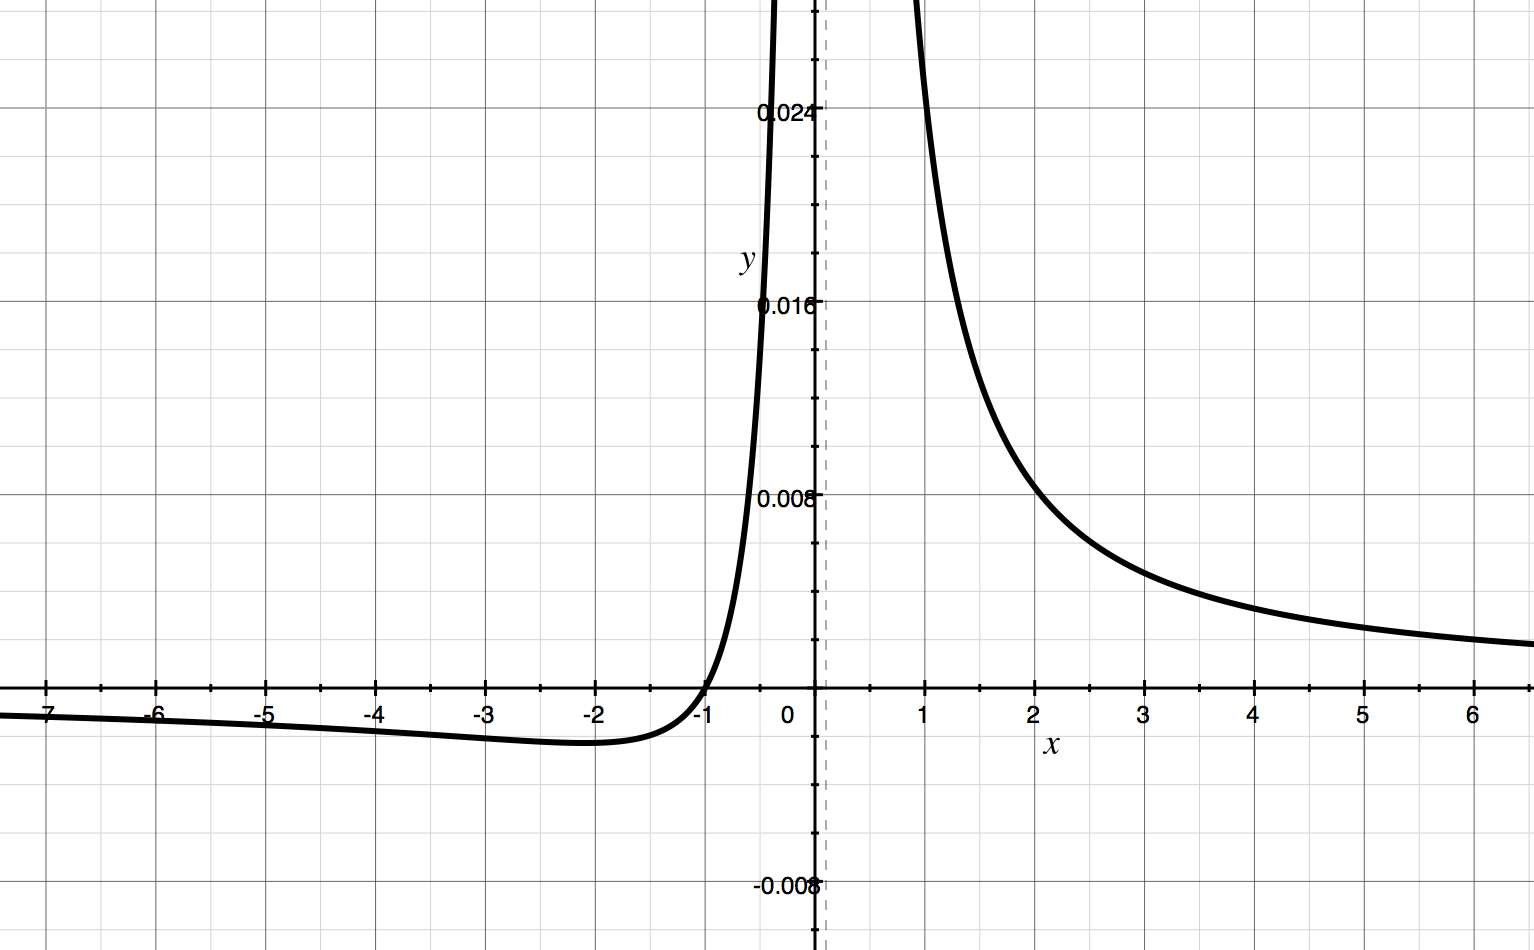
\includegraphics[scale=0.3]{\chapdir/pics/verticalasymptote}
\caption{An appropriately zoomed in graph of $\frac{x+1}{(10x-1)^2}$}
\end{centering}
\end{figure}

With this much more appropriate window, we can see that there is a local minimum,
perhaps in the vicinity of $x=-2$.  If it indeed occurs at a rational number, there is no
reason to find the derivative by hand with the TI-8* will do it for us!

\index{TI-8*!graph derivatives}
Set $Y_2$ to be \texttt{nDeriv(Y$_1$(X),X,X)} or $\left.\frac{d}{dx}(Y_1(X))\right|_{X=X}$, 
depending upon your model of TI-8*.  (nDerive is choice 8 under 
\Touche[style=function,principal=math].)  It seems have a
zero near 2.  The function is clearly concave and derivative is increasing, so it should be
a local minimum.  Using ZERO (under 
\Touche[style=function,principal=trace,fontsize=7pt,position=0.9]
), we find it to be exactly -2.1.  Plugging
back into the original equation, we get $\frac{-1.1}{484}$, which $\triangleright$FRAC
converts to $-\frac{1}{440}$.
